\documentclass[a4paper, english]{article}
\setlength{\columnsep}{20pt}
\usepackage[utf8]{inputenc}
\usepackage{algorithm} 
\usepackage{algpseudocode}
\usepackage{listings}
\usepackage{xcolor}
%\usepackage{url}
%\usepackage{algorithmic}
\usepackage{multicol}
\usepackage[a4paper]{geometry}
\usepackage{datetime}
\usepackage[font=small,labelfont=it]{caption}
\usepackage{graphicx}
\usepackage{mathpazo} % use palatino
\usepackage[scaled]{helvet} % helvetica
\usepackage{microtype}
\usepackage{amsmath}
\usepackage{subfigure}
\usepackage{float}
\usepackage{url}

%New colors defined below
\definecolor{codegreen}{rgb}{0,0.6,0}
\definecolor{codegray}{rgb}{0.5,0.5,0.5}
\definecolor{codepurple}{rgb}{0.58,0,0.82}
\definecolor{backcolour}{rgb}{0.95,0.95,0.92}

%Code listing style named "mystyle"
\lstdefinestyle{mystyle}{
  backgroundcolor=\color{backcolour},   commentstyle=\color{codegreen},
  keywordstyle=\color{magenta},
  numberstyle=\tiny\color{codegray},
  stringstyle=\color{codepurple},
  basicstyle=\ttfamily\footnotesize,
  breakatwhitespace=false,         
  breaklines=true,                 
  captionpos=b,                    
  keepspaces=true,                 
  numbers=left,                    
  numbersep=5pt,                  
  showspaces=false,                
  showstringspaces=false,
  showtabs=false,                  
  tabsize=2
}

%"mystyle" code listing set
\lstset{style=mystyle}

% Letterspacing macros
\newcommand{\spacecaps}[1]{\textls[200]{\MakeUppercase{#1}}}
\newcommand{\spacesc}[1]{\textls[50]{\textsc{\MakeLowercase{#1}}}}

\title{\spacecaps{Noise reduction using bilateral filtering}\\ \normalsize \spacesc{Edge Preserved Image Smoothing} }

\author{Shaon Rahman\\sha\_on@yahoo.com\\University of Stavanger, Norway}
%\date{\today\\\currenttime}
\date{\today}

\begin{document}

\renewcommand{\abstractname}{Summary}
\maketitle
% \begin{multicols}{1}
\begin{abstract}
%
In this project we implement Bilateral Filtering\cite{710815} and experiment on different images to see how well it performs in terms of denoising image while preserving the edges. First we describe the theory behind bilateral filtering and the idea behind it and compare with gaussian filtering. We apply `salt and pepper' and `gaussian' noise on the different test images and then filter using bilateral filter, gaussian filter\cite{wiki:gaussianfilter} compare results with each other. We experiment with different parameters of each of the filtering methods. For comparing the quality of the image after filtering we use structural similarity index\cite{wang2003ssim} to quantify structural degradation of the filtered image with the pre-noised image as the reference. We also measure peak signal-to-noise\cite{poobathy2014edge} ratio to quantify absolute difference between the reference image and the filtered image. Finally we visualize the results by plotting the structural similarity index and peak signal-to-noise ratio from our experiments.

%
\end{abstract}


\section{Introduction}
%
%The introduction is there to set the stage and define the subject of the report. It should also answer the following questions: \emph{Why is the lab performed? What is the specific purpose of this lab? Why is this lab important?}. It carries on where the abstract stopped but focuses on the topic itself. No results nor any background.
Image noise is random variation of brightness or color information in images, and is usually an aspect of electronic noise. It can be produced by the image sensor and circuitry of a scanner or digital camera. Image noise can also originate in film grain and in the unavoidable shot noise of an ideal photon detector.\cite{wiki:imagenoise} There are many techniques to reduce image noise while taking a photo by shooting with lower iso's while theres less light in the scene in the expense of longer exposure or wider aperture. After the photo is taken the image is often blurred to reduce the noise. The problem with standard blurring methods is the edges in the image gets softer after applying the blur as blurring combines the neighbours of a pixel with some weight as the function of distance of the neighbouring pixels to produce the new pixel. The edges have high contrast so when a blurring filter is applied to an edge pixel the neighbouring pixels which are radiometrically different than the edge pixel combined together softens the edge pixel overall making the edge softer. Bilateral filter tries preserve the edges by incorporating the radiometric difference of each neighbour pixel along with the euclidean distance as a factor to calculate weight for the filter. By doing so the effect of neighbouring pixels which are significantly different in values is reduced so the edges can remain sharper compared to simple filtering.

\section{Theory}
%The section \textit{Background} should provide a description of every task you implemented. It should take up about 1 A4 page if you aim at a grade 3, 1.5 A4 pages for a 4 and about 2 A4 pages if you aim at a 5 (excluding Figures). You give in this section a more detailed description of what you have implemented in this lab. You can use 2-3 figures to support your description. If you find other work which can be referenced, this would be a good place to put it.
A new pixel in bilateral filtering is calculated using following equation\cite{wiki:bilateralfiltering}


$$
I^\text{'}(x) = \frac{\sum_{x_i \in \Omega} I(x_i)f_r(\|I(x_i) - I(x)\|)g_s(\|x_i - x\|)}{W_p}
$$

where normalization term, $W_p$ is defined as,
$$
W_p = \sum_{x_i \in \Omega}{f_r(\|I(x_i) - I(x)\|)g_s(\|x_i - x\|)}
$$

Where $I^{'}$ is the filtered image,
$I$ is the input image,
$x$ is the coordinate of the current pixel,
$\Omega$ is the window centered in $x$,
$x_i \in \Omega$ is a neighbouring pixel of $x$,
$f_r$ is a function to smooth the difference of two pixel values.
$g_s$ is is a function to smooth the difference of two pixels spatial.


bilateral filter uses both spatial and range kernel two determine weight of the neighbouring pixels unlike gaussian filter\cite{wiki:gaussianfilter} which only considers the spatial distance. The range kernel is useful for preserving edges as neighbouring pixels with widely different values are assigned less weight than the neighbour thats closer in range. Bilateral filter internaly might use gaussian function for $f_r$ and $g_s$ functions. The reason to use gaussian is its inversely proportional to distance between two points or simply difference between two values. It also has a parameter sigma which can be useful to control the strength of each of the kernel. So its an ideal candidate for the task as we want the farther neighbour or the pixels with higher difference in range to have less weight in the calculation of center pixel.


if we use gaussian kernel for both the distance and range kernel we can simplify this part of equation
$
f_r(\|I(x_i) - I(x)\|)g_s(\|x_i - x\|)
$
to calculate the weight of the neighbouring pixel. The simplified equation 

$$
w(i, j, k, l) = \exp\left(-\frac{(i - k)^2 + (j - l)^2}{2 \sigma_d^2} - \frac{\|I(i, j) - I(k, l)\|^2}{2 \sigma_r^2}\right)
$$

where $i,j$ is the center pixels coordinate and $k,l$ is the neighbouring pixel and $\sigma_r, \sigma_d$ are the smoothing parameter for range and distance. So the new Image is given by
$$
I_D(i, j) = \frac{\sum_{k, l} I(k, l) w(i, j, k, l)}{\sum_{k, l} w(i, j, k, l)}
$$


\section{Implementation}
%
We implement the algorithm in Python programming language. The source code of the implementation is listed in listing \ref{bilateralfiltering}. The time complexity of the algorithm is $O(hwk^2)$ where $h$ is the height, $w$ is the width of the image and $k$ is the size of the window. The algorithm takes the original \textit{image}, the \textit{kernerl size}, and the smoothing parameters \textit{sigma color} and \textit{sigma distance} for input. We implement bilateral filtering by going over each of the pixels in the source image to calculate the new value for the pixel.

Lets call the pixel we are calculating the value `center pixel' for the purposes of explanation. The center pixel is calculated based on the summation of its neighbouring pixels within the window. Each neighbouring pixel also has a weight that determines how much it affects in the calculation of center pixel. The weight is determined based on how far the neighbouring pixel is from the center pixel. We calculate euclidean distance between the coordinates of center pixel and the neighbouring pixel and pass it to the gaussian function along with the smoothing parameter for spatial distance. As we described earlier, the bilateral filtering method also depends on the closeness of value of neighbouring pixel and the center pixel. For that we also calculate the absolute difference between the neighbouring pixel and center pixel and pass it to the gaussian function with smoothing parameter for color. The weight for spatial distance and range are multiplied together to produce final weight for that neighbouring pixel. We can control the smoothing parameters to specify how much each of the two kernels should affect the final calculation of weight. 

\section{Experiments and Results}

We use the source code in Appendix B for helping with our experimentation and comparison with Gaussian smoothing method. We will use PSNR\cite{wiki:psnr} which is a floating value in the range of 0 to infinity and SSIM\cite{wang2003ssim} which is also a floating point value in the range of 0 to 1. Both of the measurements are comparative so we take measurements after adding noise and applying filter and in both of the cases we compare the noisy image and the filtered image with the original image to measure how much quality we have lost after applying the noise and how much quality we have gained after applying the filter.

SSIM is a perception-based model that considers image degradation as perceived change in structural information, while also incorporating important perceptual phenomena, including both luminance masking and contrast masking terms\cite{wiki:ssim_wiki}. Its an important metric to evaluate edge preservation capability of an method. PSNR in other hand shows the amount of noise present in the image. A heavily smoothed image would not have much noise but It will also lose significant amout of features in the smoothing process. Thats why both of the measures are important in our case. We use following three images for our experiments. These images are also added to the appendix. A lower value signifies better quality in the measurements.

\begin{figure}[h]
\centering
    \subfigure[]{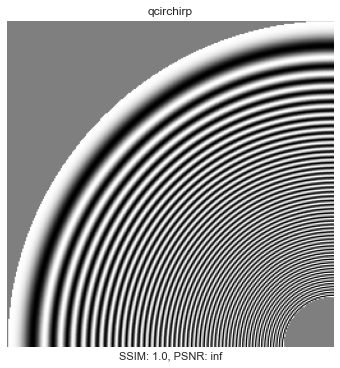
\includegraphics[width=.32\linewidth]{fig/qcirchirp.png}\label{fig:demo-standard}}
    \subfigure[]{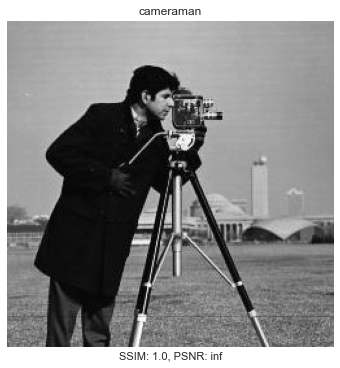
\includegraphics[width=.32\linewidth]{fig/cameraman.png}\label{fig:demo-fancy}}
    \subfigure[]{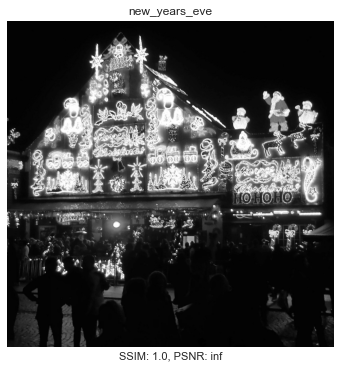
\includegraphics[width=.32\linewidth]{fig/new_years_eve.png}\label{fig:demo-fancy}}
    \caption{The set of images to run experiments on. In each of the picture our metrics are shown below. These are unmodified image, so these images have highest quality measure.}
\end{figure}

In each of the modified images (noised or denoised) the top of the image will show what method was used to generate the image and with what parameter. In the filtering parameters $k$ signifies the size of the kernel window that was used for filtering and \textit{sig} is short for $\sigma$. We wrote the ExperimentHelper class to assist in the experiments. This class will allow us to run different experiments with minimal amount of setup code. The class is listed in \textit{Listing 2}. A sample use case of the class is shown in \textit{Listing 3}

\begin{figure}[H]
\centering
    \subfigure[]{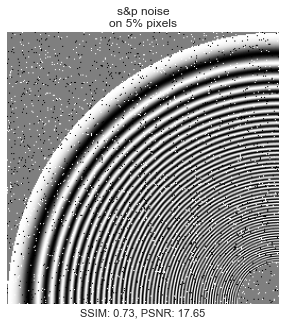
\includegraphics[width=.4\linewidth]{fig/qcirchirp_snp5.png}\label{fig:demo-standard}}
    \subfigure[]{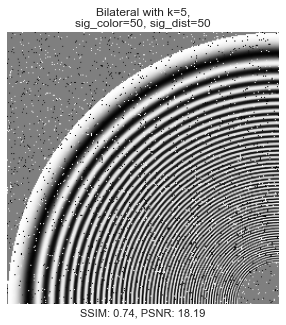
\includegraphics[width=.4\linewidth]{fig/qcirchirp_snp5_bilfil.png}\label{fig:demo-fancy}}
    \caption{The left image has 5\% salt and pepper noise and the right image is filtered with bilateral filtering method.}
\end{figure}

\begin{figure}[H]
\centering
    \subfigure[]{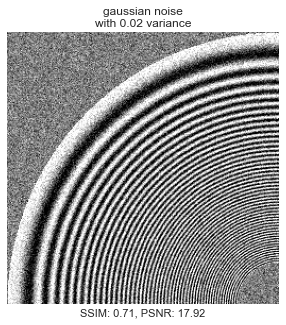
\includegraphics[width=.4\linewidth]{fig/qcirchirp_gaussian002.png}\label{fig:demo-standard}}
    \subfigure[]{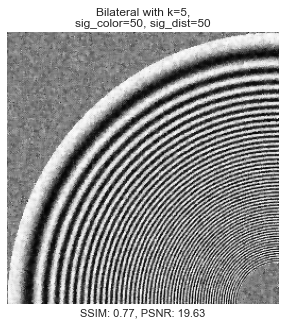
\includegraphics[width=.4\linewidth]{fig/qcirchirp_gaussian5.png}\label{fig:demo-fancy}}
    \caption{The left image has gaussin noise with 0.02 variance and 0 mean and the right image is filtered with bilateral filtering method.}
\end{figure}


We begin the experiment with qcirchirp image. We add salt and paper and gaussian noise to the image and then apply bilateral filtering and calculate the metrics. We see in both of the cases the quality measures have improved significantly after filtering the images.


We now compare bilateral filtering with gaussian smoothing\cite{wiki:gaussianfilter}. Gaussian filter only consideres the distances of the neighbouring pixels when calculating the weight of the center pixel where bilateral filtering takes the spatial distance and the similarity of neighbouring pixel into account which helps it preserves edges. To find out how much of the range component helps bilateral filtering in preserving edges we add harsher noise to the image and apply stronger filter.

\begin{figure}[H]
\centering
    \subfigure[]{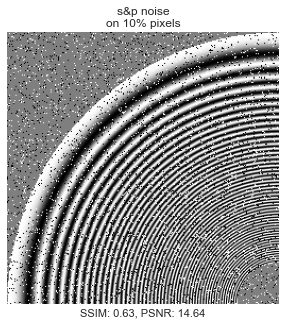
\includegraphics[width=.32\linewidth]{fig/qcirchirp_snp10.png}\label{fig:demo-standard}}
    \subfigure[]{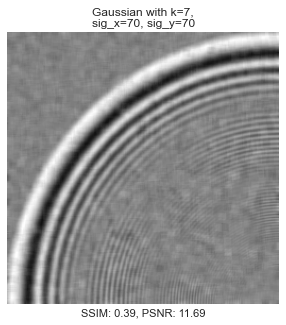
\includegraphics[width=.32\linewidth]{fig/qcirchirp_snp10_gauss.png}\label{fig:demo-fancy}}
    \subfigure[]{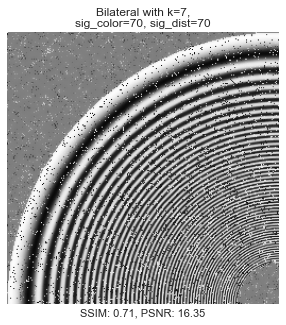
\includegraphics[width=.32\linewidth]{fig/qcirchirp_snp10_bifi.png}\label{fig:demo-fancy}}
    \caption{Noisy Image filtered with gaussian filter and bilateral filter}
\end{figure}

Image (a) has salt and paper noise in 10\% of the pixels, (a) is filtered with gaussian filter(b) and bilateral filter(c). We can see gaussian filter did not do very well in this case. The gaussian filter reduced the metrics even more than the noisy image while bilateral filtering has increased both of the metrics significantly. The SSIM score has been significantly improved in image (c). Its because the bilateral filter denoised the image while preserving the edges. It can be visually seen that image (b) lost a lot of its structures in the high frequency waves in the image.

We now see how bilateral filter compares with gaussian filter in gaussian reducing gaussian noise.

\begin{figure}[H]
\centering
    \subfigure[]{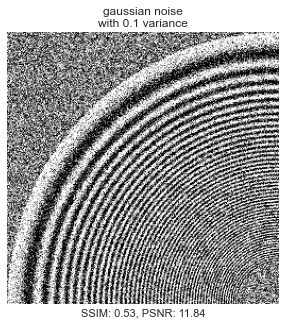
\includegraphics[width=.32\linewidth]{fig/qcirchirp_gauss01.png}\label{fig:demo-standard}}
    \subfigure[]{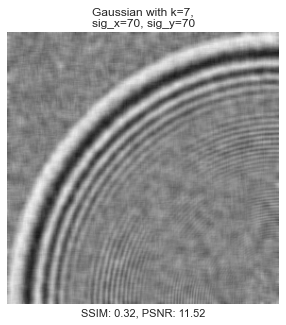
\includegraphics[width=.32\linewidth]{fig/qcirchirp_gauss01_gauss.png}\label{fig:demo-fancy}}
    \subfigure[]{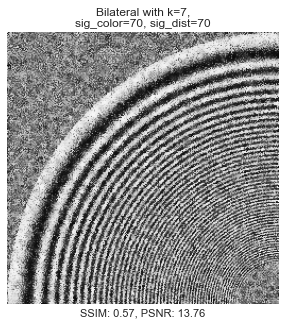
\includegraphics[width=.32\linewidth]{fig/qcirchirp_gauss01_bifi.png}\label{fig:demo-fancy}}
    \caption{Noisy Image filtered with gaussian filter and bilateral filter}
\end{figure}

Now that we have seen that the bilateral filtering method is clearly superior than the gaussian filter in retaining structure of the image while smoothing the noise\footnote{Experimentation with other images are attached in Appendix}. we experiment with the values of parameters in bilateral filtering. For this experiment we Filter the image in \textit{Figure 4 (a)} which has salt and paper noise and \textit{Figure 5 (a)} which has gaussian noise. We filter this images with values of $30, 80, 130$ for $\sigma_r$ and $\sigma_d$ parameters of bilateral filtering and we fix the kernel size to $7$. The results of the experiment is attached in the \textit{Appendix A3}. In both of the cases we see a lower value of $\sigma_r$ got higher scores. In the image with salt paper noise the image (e) has the highest psnr and ssim it was filtered with $\sigma_r = 80$ and $\sigma_d = 80$ for gaussian noise the filter with same parameters performed well. The gaussian noise is harder to smooth because every pixel is modified in gaussian noise unlike salt and paper noise.

To see how much each $\sigma$ parameters affect the quality metrics, we fix one of the parameter and experiment with changing the other and plot our results. We first perform this experiment with salt and paper noise on 10\% pixels.

\begin{figure}[H]
\centering
    \subfigure[]{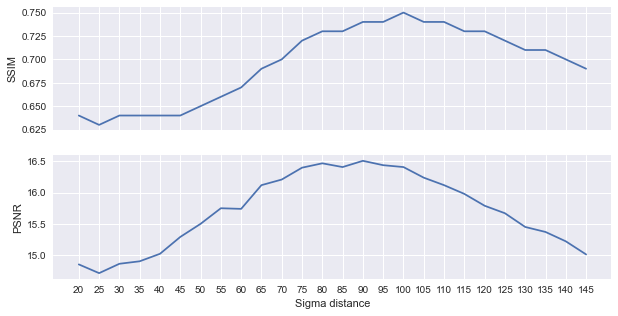
\includegraphics[width=1\linewidth]{fig/metrics_plot_fixed_ss.png}}
    \caption{Evaluation metrics over different values of $\sigma_d$}
\end{figure}

We see that the best result is found when $\sigma_d = 5$ fixing $\sigma_r = 80$. Now we freeze $\sigma_d = 80$ and see how $\sigma_r$ affects our results.

\begin{figure}[H]
\centering
    \subfigure[]{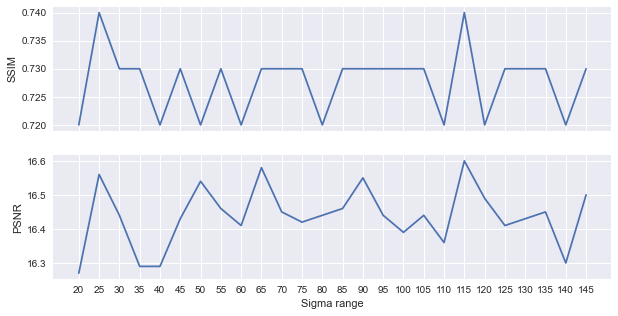
\includegraphics[width=1\linewidth]{fig/metrics_plot_fixed_sc.png}}
    \caption{Evaluation metrics over different values of $\sigma_r$}
\end{figure}

From this experiment we can see that the range parameter is not as consistent as the distance parameter. Experimenting with different images we can also see it depends heavily from image to image which makes sense as the range parameter depends on values on neighbouring pixel which can vary a lot compared to distance which is quite consistent. Now we perform the same experiment with gaussian noise.

\begin{figure}[H]
\centering
    \subfigure[]{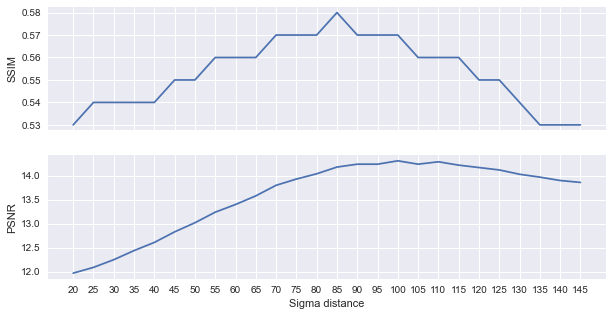
\includegraphics[width=1\linewidth]{fig/metrics_plot_fixed_ss_gauss.png}}
    \caption{Evaluation metrics over different values of $\sigma_d$}
\end{figure}

Freezing $\sigma_d = 80$,

\begin{figure}[H]
\centering
    \subfigure[]{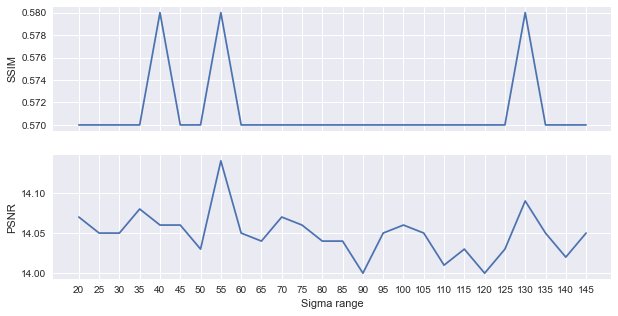
\includegraphics[width=1\linewidth]{fig/metrics_plot_fixed_sc_gauss.png}}
    \caption{Evaluation metrics over different values of $\sigma_r$}
\end{figure}

We see a similar case in gaussian noise filtering as well. We also note that changing only one parameter at a time doesnt have a significant amount of effect on the quality of the image which is by design as the normalizing term which is calculated based on the range and distance kernel normalizes the overall effect on the image.

\section{Conclusion}
From our experiments we saw how well Bilateral Filtering works compared to Gaussian filter. We saw how the parameters of bilateral filtering affects different images with different types of noise. We saw that its vastly superior in images with lot of edges and in smooth surfaces it works just like the gaussian filter. 

Experimenting with different parameters of the bilateral filtering we found that tuning the distance parameter produces more consistent result than tuning the range parameter. The range parameter depends from image to image while the distance parameter is consistent in all images. That is because the pixel values can be significantly different than one another while the distance from the center pixel to the neighbouring pixels are consistent.

\nocite{*}
% \end{multicols}
\bibliographystyle{plain}
\bibliography{references}

\appendix

\section{Images}
\subsection{The original Images}
\centering
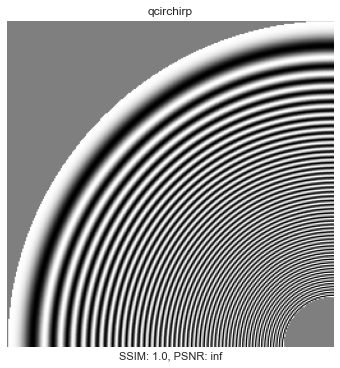
\includegraphics[width=.6\linewidth]{fig/qcirchirp.png}\\
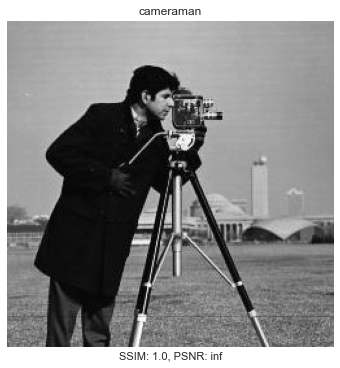
\includegraphics[width=.6\linewidth]{fig/cameraman.png}\\
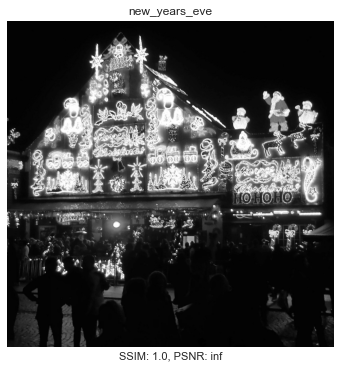
\includegraphics[width=.6\linewidth]{fig/new_years_eve.png}

\subsection{Comparison of gaussian and bilateral filtering}
\begin{figure}[H]
\centering
    \subfigure[]{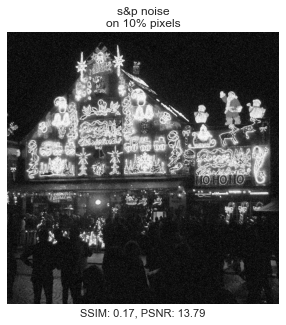
\includegraphics[width=.32\linewidth]{fig/new_years_eve_snp10.png}\label{fig:demo-standard}}
    \subfigure[]{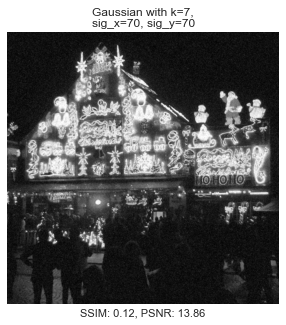
\includegraphics[width=.32\linewidth]{fig/new_years_eve_snp10_gauss.png}\label{fig:demo-fancy}}
    \subfigure[]{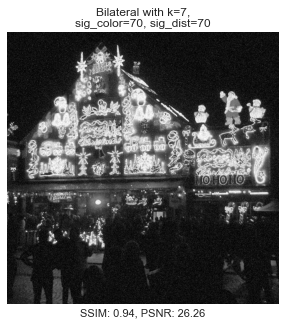
\includegraphics[width=.32\linewidth]{fig/new_years_eve_snp10_bifi.png}\label{fig:demo-fancy}}
    \caption{Noisy Image filtered with gaussian filter and bilateral filter}
\end{figure}

\begin{figure}[H]
\centering
    \subfigure[]{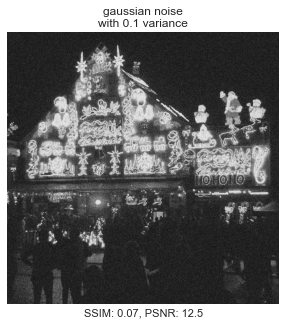
\includegraphics[width=.32\linewidth]{fig/new_years_eve_gauss01.png}\label{fig:demo-standard}}
    \subfigure[]{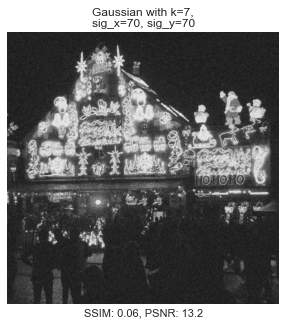
\includegraphics[width=.32\linewidth]{fig/new_years_eve_gauss01_gauss.png}\label{fig:demo-fancy}}
    \subfigure[]{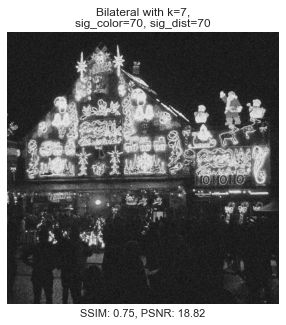
\includegraphics[width=.32\linewidth]{fig/new_years_eve_gauss01_bifi.png}\label{fig:demo-fancy}}
    \caption{Noisy Image filtered with gaussian filter and bilateral filter}
\end{figure}

\begin{figure}[H]
\centering
    \subfigure[]{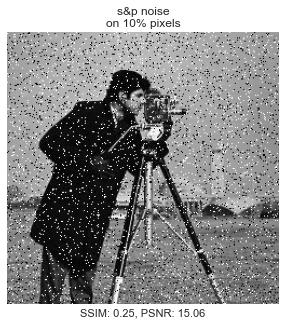
\includegraphics[width=.32\linewidth]{fig/cameraman_snp10.png}\label{fig:demo-standard}}
    \subfigure[]{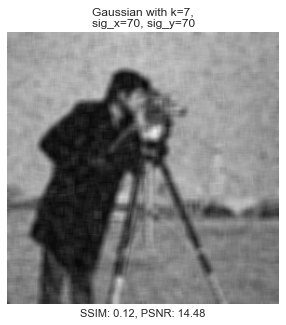
\includegraphics[width=.32\linewidth]{fig/cameraman_snp10_gauss.png}\label{fig:demo-fancy}}
    \subfigure[]{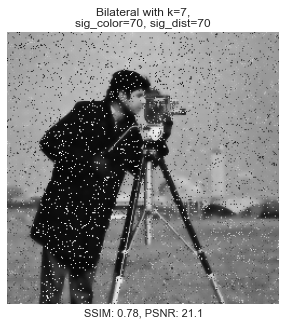
\includegraphics[width=.32\linewidth]{fig/cameraman_snp10_bifi.png}\label{fig:demo-fancy}}
    \caption{Noisy Image filtered with gaussian filter and bilateral filter}
\end{figure}

\begin{figure}[H]
\centering
    \subfigure[]{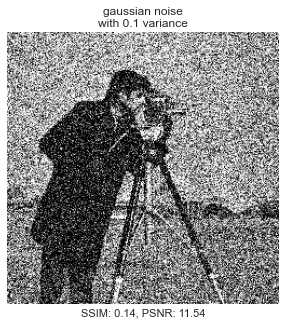
\includegraphics[width=.32\linewidth]{fig/cameraman_gauss01.png}\label{fig:demo-standard}}
    \subfigure[]{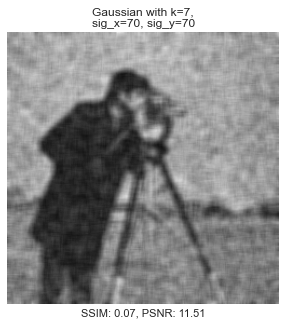
\includegraphics[width=.32\linewidth]{fig/cameraman_gauss01_gauss.png}\label{fig:demo-fancy}}
    \subfigure[]{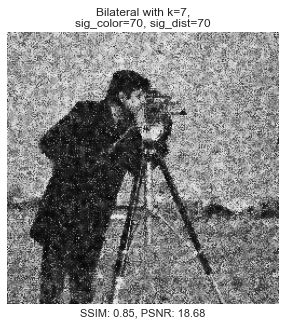
\includegraphics[width=.32\linewidth]{fig/cameraman_gauss01_bifi.png}\label{fig:demo-fancy}}
    \caption{Noisy Image filtered with gaussian filter and bilateral filter}
\end{figure}
\newpage
\subsection{Bilater filtering with different parameters}
\subsubsection{Image with salt and paper noise}
\begin{figure}[H]
\centering
    \subfigure[]{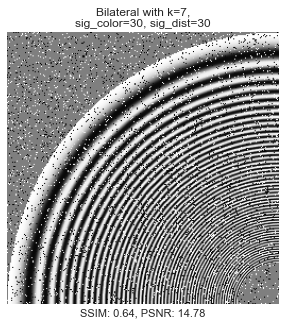
\includegraphics[width=.32\linewidth]{fig/qcirchirp_snp10_bifi_ss30_sc30.png}\label{fig:demo-standard}}
    \subfigure[]{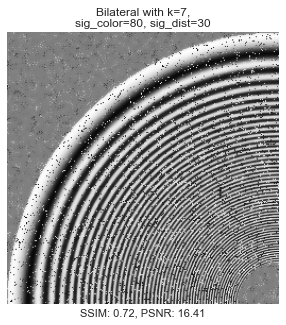
\includegraphics[width=.32\linewidth]{fig/qcirchirp_snp10_bifi_ss30_sc80.png}\label{fig:demo-standard}}
    \subfigure[]{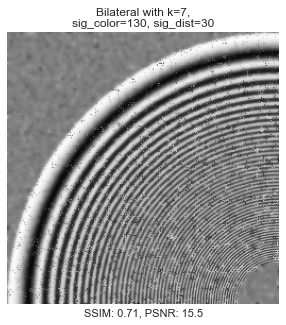
\includegraphics[width=.32\linewidth]{fig/qcirchirp_snp10_bifi_ss30_sc130.png}\label{fig:demo-standard}}
    \newline
    \subfigure[]{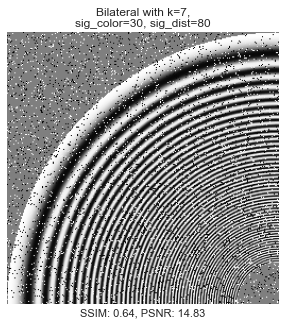
\includegraphics[width=.32\linewidth]{fig/qcirchirp_snp10_bifi_ss80_sc30.png}\label{fig:demo-standard}}
    \subfigure[]{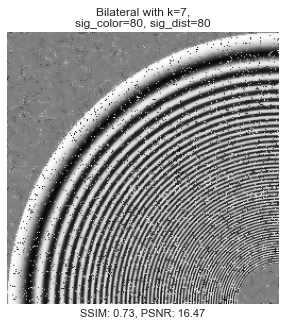
\includegraphics[width=.32\linewidth]{fig/qcirchirp_snp10_bifi_ss80_sc80.png}\label{fig:demo-standard}}
    \subfigure[]{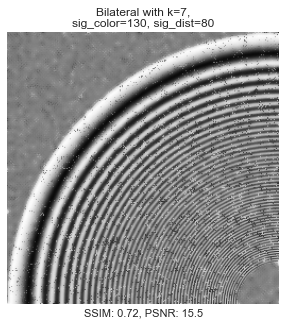
\includegraphics[width=.32\linewidth]{fig/qcirchirp_snp10_bifi_ss80_sc130.png}\label{fig:demo-standard}}
    \newline
    \subfigure[]{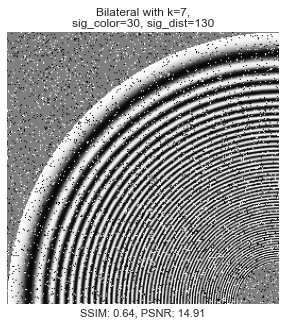
\includegraphics[width=.32\linewidth]{fig/qcirchirp_snp10_bifi_ss130_sc30.png}\label{fig:demo-standard}}
    \subfigure[]{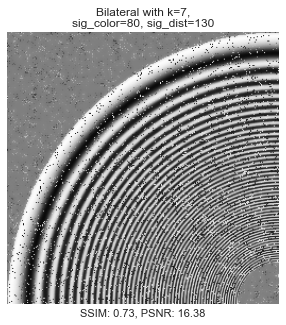
\includegraphics[width=.32\linewidth]{fig/qcirchirp_snp10_bifi_ss130_sc80.png}\label{fig:demo-standard}}
    \subfigure[]{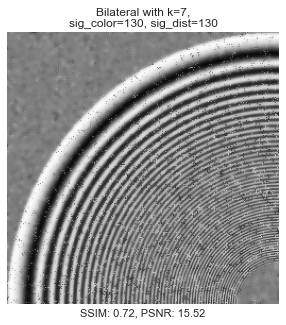
\includegraphics[width=.32\linewidth]{fig/qcirchirp_snp10_bifi_ss130_sc130.png}\label{fig:demo-standard}}
    \caption{Images filtered with different values for $\sigma_r$ and $\sigma_d$}
\end{figure}
\newpage
\subsubsection{Image with gaussian noise}
\begin{figure}[H]
\centering
    \subfigure[]{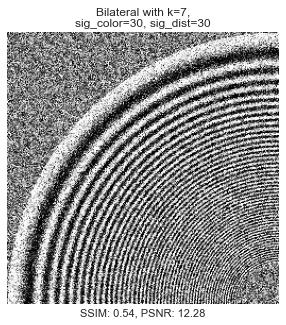
\includegraphics[width=.32\linewidth]{fig/qcirchirp_gauss01_bifi_ss30_sc30.png}\label{fig:demo-standard}}
    \subfigure[]{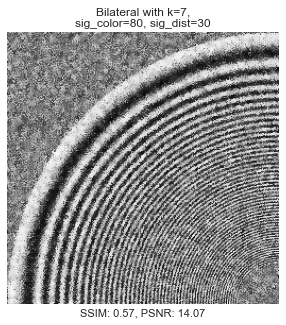
\includegraphics[width=.32\linewidth]{fig/qcirchirp_gauss01_bifi_ss30_sc80.png}\label{fig:demo-standard}}
    \subfigure[]{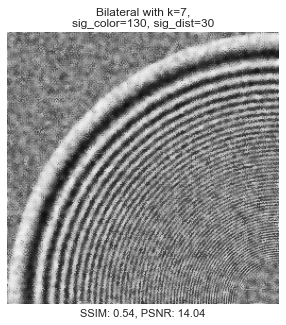
\includegraphics[width=.32\linewidth]{fig/qcirchirp_gauss01_bifi_ss30_sc130.png}\label{fig:demo-standard}}
    \newline
    \subfigure[]{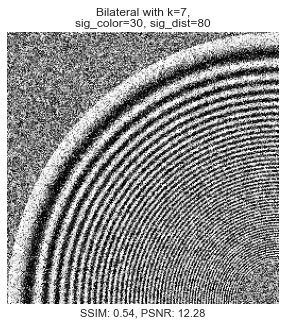
\includegraphics[width=.32\linewidth]{fig/qcirchirp_gauss01_bifi_ss80_sc30.png}\label{fig:demo-standard}}
    \subfigure[]{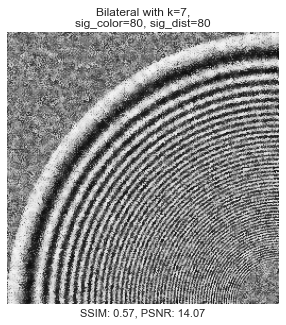
\includegraphics[width=.32\linewidth]{fig/qcirchirp_gauss01_bifi_ss80_sc80.png}\label{fig:demo-standard}}
    \subfigure[]{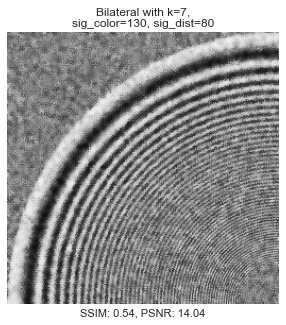
\includegraphics[width=.32\linewidth]{fig/qcirchirp_gauss01_bifi_ss80_sc130.png}\label{fig:demo-standard}}
    \newline
    \subfigure[]{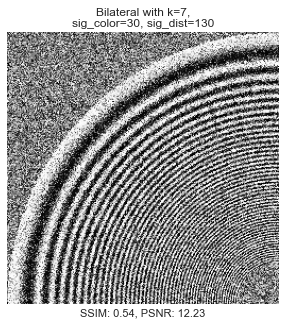
\includegraphics[width=.32\linewidth]{fig/qcirchirp_gauss01_bifi_ss130_sc30.png}\label{fig:demo-standard}}
    \subfigure[]{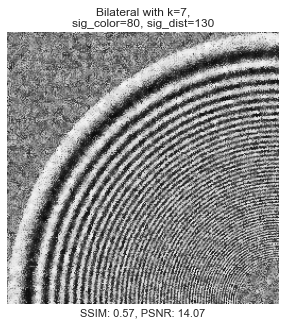
\includegraphics[width=.32\linewidth]{fig/qcirchirp_gauss01_bifi_ss130_sc80.png}\label{fig:demo-standard}}
    \subfigure[]{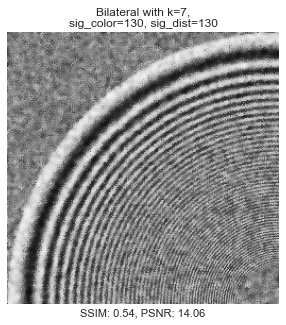
\includegraphics[width=.32\linewidth]{fig/qcirchirp_gauss01_bifi_ss130_sc130.png}\label{fig:demo-standard}}
    \caption{Images filtered with different values for $\sigma_r$ and $\sigma_d$}
\end{figure}
\newpage
\section{Source codes}

All the codes for this project can be found in the following github repository
\centering
    \begin{verbatim}
    https://github.com/Wizdore/Bilateral-Filtering_image_processing_project
    \end{verbatim}

\subsection{Bilateral Filtering Python Source Code}
\begin{lstlisting}[language=Python, caption=Bilateral Filtering function, label=bilateralfiltering]
def bilateral_filter(IMAGE, kernel_size, SIGMA_DISTANCE, SIGMA_RANGE):
    """
    Bilateral filters an Image
    :param IMAGE: The source Image
    :param kernel_size: Size of the kernel window

    :param SIGMA_RANGE: Smoothing parameter for range
    :param SIGMA_DISTANCE: Smoothing parameter for distance
    :return: A Bilateral Filtered Image
    """
    d = kernel_size // 2
    img_filtered = np.zeros(IMAGE.shape, dtype=np.uint8)
    IMAGE = np.pad(IMAGE, d, 'mean')


    def filter(i, j, d):
        def calculate_weight(i, j, k, l):
            t_distance = - (np.square(i-k) + np.square(j-l))\
                         / 2 / np.square(SIGMA_DISTANCE)
            t_range = - np.square(IMAGE[i, j] - IMAGE[k, l])\
                      / 2 / np.square(SIGMA_RANGE)
            return np.exp(t_distance + t_range)

        sum_w = 0
        sum_iw = 0
        for k in range(i - d, i + d + 1):
            for l in range(j - d, j + d + 1):
                w = calculate_weight(i, j, k, l)
                sum_iw += IMAGE[k, l] * w
                sum_w += w
        return int(sum_iw / sum_w)

    for i in tqdm(range(d, IMAGE.shape[0] - d)):
        for j in range(d, IMAGE.shape[1] - d):
            img_filtered[i - d, j - d] = filter(i, j, d)
    return img_filtered

\end{lstlisting}
\newpage
\subsection{Utility code to help with experimentation}
\begin{lstlisting}[language=Python, caption=Class to streamline the experimentation process, label=experimentation_code]
class ExperimentHelper:
    def __init__(self, img):
        self.image = img
        self.original_image = img
        self.title = 'original image'
        self.psnr = float('inf')
        self.ssim = 1.0
        self.caption = f'SSIM: {self.ssim}, PSNR: {self.psnr}'
    
    #Resets the image to the original state
    def reset(self):
        self.image = self.original_image
        self.title = 'original image'
        self.psnr = float('inf')
        self.ssim = 1.0
        self.caption = f'SSIM: {self.ssim}, PSNR: {self.psnr}'
        return self

    def get_metrics(self):
        return {'psnr': self.psnr, 'ssim':self.ssim}
    
    # Compares the modified state of the image to another image
    def compare_to(self, another_image):
        psnr = peak_signal_noise_ratio(self.image,another_image, data_range=255)
        ssim, _= structural_similarity(self.image, another_image, full=True)
        return np.round(psnr, 2), np.round(ssim, 2)
    
    # display the Image at current state with generated title and caption
    # The image is also saved if save_figure_name has a string for the name
    def show(self, save_figure_name=''):
        fig = plt.figure(figsize=(6,6))
        ax = fig.add_subplot(111)
        ax.set_title(self.title)
        ax.set(xticks=[], yticks=[], xlabel=self.caption)
        plt.imshow(self.image, cmap='gray', vmin=0, vmax=255)
        if save_figure_name != '':
            plt.savefig(f'{save_figure_name}.png')
        plt.tight_layout()
        plt.show()
        return self

    # get the plot to be shown in a figure
    # Can be used for making subplots
    def get_plot(self, ax):
        ax.set_title(self.title)
        ax.set(xticks=[], yticks=[], xlabel=self.caption)
        ax.imshow(self.image, cmap='gray', vmin=0, vmax=255)
        return ax

    def add_noise(self, mode, amount=None, var=None):
        assert mode in ['s&p', 'salt', 'pepper', 'gaussian', 'poisson', 'speckle']

        noisy = np.zeros(self.image.shape)

        if mode in ['s&p', 'salt', 'pepper']:
            self.title = f'{mode} noise\non {round(amount*100)}% pixels'
            noisy = skp.random_noise(self.image, mode=mode,
                                          amount=amount, clip=True) * 255

        if mode in ['gaussian', 'poisson', 'speckle']:
            self.title = f'{mode} noise\nwith {var}% variance'
            noisy = skp.random_noise(self.image, mode=mode,
                                          var=var, clip=True) * 255

        noisy = noisy.astype(np.uint8)
        self.psnr, self.ssim = self.compare_to(noisy)
        self.caption = f'SSIM: {self.ssim}, PSNR: {self.psnr}'
        self.image = noisy
        return self

    def gaussian_filter(self, kernel, sigmaX=50, sigmaY=50):
        filtered = cv2.GaussianBlur(self.image, (kernel,kernel),
                                    sigmaX=sigmaX, sigmaY=sigmaY,
                                    borderType=cv2.BORDER_REPLICATE)
        self.psnr, self.ssim = self.compare_to(filtered)
        self.caption = f'SSIM: {self.ssim}, PSNR: {self.psnr}'
        self.title = f'Gaussian with k={kernel},\nsig_x={sigmaX}, sig_y={sigmaY}'
        self.image = filtered
        return self

    def bilateral_filter(self, kernel, sigmaColor=50, sigmaSpace=50):
        filtered = cv2.bilateralFilter(self.image, kernel,
                                       sigmaColor, sigmaSpace,
                                       borderType=cv2.BORDER_REPLICATE)
        self.psnr, self.ssim = self.compare_to(filtered)
        self.caption = f'SSIM: {self.ssim}, PSNR: {self.psnr}'
        self.title = f'Bilateral with k={kernel},\nsig_color={sigmaColor}, sig_dist={sigmaSpace}'
        self.image = filtered
        return self

\end{lstlisting}

\newpage
\subsection{Use case of ExperimentHelper Class}
\begin{lstlisting}[language=Python, caption=A sample use case of the class, label=experimentation_code_use]
# We load the Image on our experiment object
img = cv2.imread('images/qcirchirp.bmp', cv2.IMREAD_GRAYSCALE)
exp3 = ExperimentHelper(img, title='qcirchirp')

# In the following lines: 
# we add noise to the image using add_noise
# display the image and save the figure with a name
# apply bilateral filter with given parameter to noisy image
# show the image but dont save it as a figure
# reset the image to the original image
# we add gaussian noise 
# and so on
# return the psnr and ssim as a dictionary compared to the original image

metrics =exp3.add_noise(mode='s&p', amount=0.1)\
    .show(save_figure_name='qcirchirp_snp10')\
    .bilateral_filter(kernel=7, sigmaColor=70, sigmaSpace=70)\
    .show()\
    .reset()\
    .add_noise(mode='gaussian', var=0.1)\
    .show()\
    .gaussian_filter(kernel=7, sigmaX=70, sigmaY=70)\
    .show()\
    .get_metrics()

# These operations can be stacked and mismatched together to create different 
# Comparisons with the original image and the final modified version of the image.
# There are more methods in the class which has not been shown here but are described
# within the comments in each function.

# we print out the metrics
print(metrics['psnr'], metrics['ssim'])
\end{lstlisting}


\end{document}

